% Created by tikzDevice version 0.12
% !TEX encoding = UTF-8 Unicode
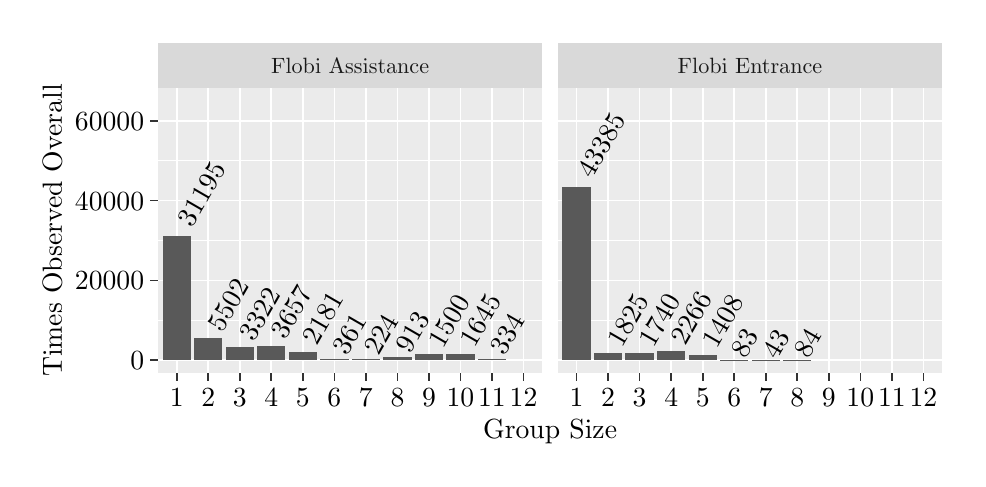
\begin{tikzpicture}[x=1pt,y=1pt]
\definecolor{fillColor}{RGB}{255,255,255}
\path[use as bounding box,fill=fillColor,fill opacity=0.00] (0,0) rectangle (336.00,155.74);
\begin{scope}
\path[clip] (  0.00,  0.00) rectangle (336.00,155.74);
\definecolor{drawColor}{RGB}{255,255,255}
\definecolor{fillColor}{RGB}{255,255,255}

\path[draw=drawColor,line width= 0.6pt,line join=round,line cap=round,fill=fillColor] (  0.00,  0.00) rectangle (336.00,155.74);
\end{scope}
\begin{scope}
\path[clip] ( 47.03, 30.86) rectangle (186.01,133.98);
\definecolor{fillColor}{gray}{0.92}

\path[fill=fillColor] ( 47.03, 30.86) rectangle (186.01,133.98);
\definecolor{drawColor}{RGB}{255,255,255}

\path[draw=drawColor,line width= 0.3pt,line join=round] ( 47.03, 49.97) --
	(186.01, 49.97);

\path[draw=drawColor,line width= 0.3pt,line join=round] ( 47.03, 78.82) --
	(186.01, 78.82);

\path[draw=drawColor,line width= 0.3pt,line join=round] ( 47.03,107.66) --
	(186.01,107.66);

\path[draw=drawColor,line width= 0.6pt,line join=round] ( 47.03, 35.55) --
	(186.01, 35.55);

\path[draw=drawColor,line width= 0.6pt,line join=round] ( 47.03, 64.39) --
	(186.01, 64.39);

\path[draw=drawColor,line width= 0.6pt,line join=round] ( 47.03, 93.24) --
	(186.01, 93.24);

\path[draw=drawColor,line width= 0.6pt,line join=round] ( 47.03,122.08) --
	(186.01,122.08);

\path[draw=drawColor,line width= 0.6pt,line join=round] ( 53.86, 30.86) --
	( 53.86,133.98);

\path[draw=drawColor,line width= 0.6pt,line join=round] ( 65.25, 30.86) --
	( 65.25,133.98);

\path[draw=drawColor,line width= 0.6pt,line join=round] ( 76.65, 30.86) --
	( 76.65,133.98);

\path[draw=drawColor,line width= 0.6pt,line join=round] ( 88.04, 30.86) --
	( 88.04,133.98);

\path[draw=drawColor,line width= 0.6pt,line join=round] ( 99.43, 30.86) --
	( 99.43,133.98);

\path[draw=drawColor,line width= 0.6pt,line join=round] (110.82, 30.86) --
	(110.82,133.98);

\path[draw=drawColor,line width= 0.6pt,line join=round] (122.22, 30.86) --
	(122.22,133.98);

\path[draw=drawColor,line width= 0.6pt,line join=round] (133.61, 30.86) --
	(133.61,133.98);

\path[draw=drawColor,line width= 0.6pt,line join=round] (145.00, 30.86) --
	(145.00,133.98);

\path[draw=drawColor,line width= 0.6pt,line join=round] (156.39, 30.86) --
	(156.39,133.98);

\path[draw=drawColor,line width= 0.6pt,line join=round] (167.78, 30.86) --
	(167.78,133.98);

\path[draw=drawColor,line width= 0.6pt,line join=round] (179.18, 30.86) --
	(179.18,133.98);
\definecolor{fillColor}{gray}{0.35}

\path[fill=fillColor] ( 48.73, 35.55) rectangle ( 58.99, 80.54);

\path[fill=fillColor] ( 60.13, 35.55) rectangle ( 70.38, 43.48);

\path[fill=fillColor] ( 71.52, 35.55) rectangle ( 81.77, 40.34);

\path[fill=fillColor] ( 82.91, 35.55) rectangle ( 93.16, 40.82);

\path[fill=fillColor] ( 94.30, 35.55) rectangle (104.56, 38.70);

\path[fill=fillColor] (105.70, 35.55) rectangle (115.95, 36.07);

\path[fill=fillColor] (117.09, 35.55) rectangle (127.34, 35.87);

\path[fill=fillColor] (128.48, 35.55) rectangle (138.73, 36.87);

\path[fill=fillColor] (139.87, 35.55) rectangle (150.13, 37.71);

\path[fill=fillColor] (151.27, 35.55) rectangle (161.52, 37.92);

\path[fill=fillColor] (162.66, 35.55) rectangle (172.91, 36.03);
\definecolor{drawColor}{RGB}{0,0,0}

\node[text=drawColor,rotate= 60.00,anchor=base west,inner sep=0pt, outer sep=0pt, scale=  1.00] at ( 59.36, 83.16) {31195};

\node[text=drawColor,rotate= 60.00,anchor=base west,inner sep=0pt, outer sep=0pt, scale=  1.00] at ( 70.25, 45.23) {5502};

\node[text=drawColor,rotate= 60.00,anchor=base west,inner sep=0pt, outer sep=0pt, scale=  1.00] at ( 81.65, 42.09) {3322};

\node[text=drawColor,rotate= 60.00,anchor=base west,inner sep=0pt, outer sep=0pt, scale=  1.00] at ( 93.04, 42.57) {3657};

\node[text=drawColor,rotate= 60.00,anchor=base west,inner sep=0pt, outer sep=0pt, scale=  1.00] at (104.43, 40.44) {2181};

\node[text=drawColor,rotate= 60.00,anchor=base west,inner sep=0pt, outer sep=0pt, scale=  1.00] at (115.32, 36.95) {361};

\node[text=drawColor,rotate= 60.00,anchor=base west,inner sep=0pt, outer sep=0pt, scale=  1.00] at (126.71, 36.75) {224};

\node[text=drawColor,rotate= 60.00,anchor=base west,inner sep=0pt, outer sep=0pt, scale=  1.00] at (138.11, 37.75) {913};

\node[text=drawColor,rotate= 60.00,anchor=base west,inner sep=0pt, outer sep=0pt, scale=  1.00] at (150.00, 39.46) {1500};

\node[text=drawColor,rotate= 60.00,anchor=base west,inner sep=0pt, outer sep=0pt, scale=  1.00] at (161.39, 39.67) {1645};

\node[text=drawColor,rotate= 60.00,anchor=base west,inner sep=0pt, outer sep=0pt, scale=  1.00] at (172.28, 36.91) {334};
\end{scope}
\begin{scope}
\path[clip] (191.51, 30.86) rectangle (330.50,133.98);
\definecolor{fillColor}{gray}{0.92}

\path[fill=fillColor] (191.51, 30.86) rectangle (330.50,133.98);
\definecolor{drawColor}{RGB}{255,255,255}

\path[draw=drawColor,line width= 0.3pt,line join=round] (191.51, 49.97) --
	(330.50, 49.97);

\path[draw=drawColor,line width= 0.3pt,line join=round] (191.51, 78.82) --
	(330.50, 78.82);

\path[draw=drawColor,line width= 0.3pt,line join=round] (191.51,107.66) --
	(330.50,107.66);

\path[draw=drawColor,line width= 0.6pt,line join=round] (191.51, 35.55) --
	(330.50, 35.55);

\path[draw=drawColor,line width= 0.6pt,line join=round] (191.51, 64.39) --
	(330.50, 64.39);

\path[draw=drawColor,line width= 0.6pt,line join=round] (191.51, 93.24) --
	(330.50, 93.24);

\path[draw=drawColor,line width= 0.6pt,line join=round] (191.51,122.08) --
	(330.50,122.08);

\path[draw=drawColor,line width= 0.6pt,line join=round] (198.35, 30.86) --
	(198.35,133.98);

\path[draw=drawColor,line width= 0.6pt,line join=round] (209.74, 30.86) --
	(209.74,133.98);

\path[draw=drawColor,line width= 0.6pt,line join=round] (221.13, 30.86) --
	(221.13,133.98);

\path[draw=drawColor,line width= 0.6pt,line join=round] (232.53, 30.86) --
	(232.53,133.98);

\path[draw=drawColor,line width= 0.6pt,line join=round] (243.92, 30.86) --
	(243.92,133.98);

\path[draw=drawColor,line width= 0.6pt,line join=round] (255.31, 30.86) --
	(255.31,133.98);

\path[draw=drawColor,line width= 0.6pt,line join=round] (266.70, 30.86) --
	(266.70,133.98);

\path[draw=drawColor,line width= 0.6pt,line join=round] (278.09, 30.86) --
	(278.09,133.98);

\path[draw=drawColor,line width= 0.6pt,line join=round] (289.49, 30.86) --
	(289.49,133.98);

\path[draw=drawColor,line width= 0.6pt,line join=round] (300.88, 30.86) --
	(300.88,133.98);

\path[draw=drawColor,line width= 0.6pt,line join=round] (312.27, 30.86) --
	(312.27,133.98);

\path[draw=drawColor,line width= 0.6pt,line join=round] (323.66, 30.86) --
	(323.66,133.98);
\definecolor{fillColor}{gray}{0.35}

\path[fill=fillColor] (193.22, 35.55) rectangle (203.47, 98.12);

\path[fill=fillColor] (204.61, 35.55) rectangle (214.87, 38.18);

\path[fill=fillColor] (216.01, 35.55) rectangle (226.26, 38.06);

\path[fill=fillColor] (227.40, 35.55) rectangle (237.65, 38.82);

\path[fill=fillColor] (238.79, 35.55) rectangle (249.04, 37.58);

\path[fill=fillColor] (250.18, 35.55) rectangle (260.44, 35.67);

\path[fill=fillColor] (261.58, 35.55) rectangle (271.83, 35.61);

\path[fill=fillColor] (272.97, 35.55) rectangle (283.22, 35.67);
\definecolor{drawColor}{RGB}{0,0,0}

\node[text=drawColor,rotate= 60.00,anchor=base west,inner sep=0pt, outer sep=0pt, scale=  1.00] at (203.85,100.74) {43385};

\node[text=drawColor,rotate= 60.00,anchor=base west,inner sep=0pt, outer sep=0pt, scale=  1.00] at (214.74, 39.93) {1825};

\node[text=drawColor,rotate= 60.00,anchor=base west,inner sep=0pt, outer sep=0pt, scale=  1.00] at (226.13, 39.81) {1740};

\node[text=drawColor,rotate= 60.00,anchor=base west,inner sep=0pt, outer sep=0pt, scale=  1.00] at (237.53, 40.57) {2266};

\node[text=drawColor,rotate= 60.00,anchor=base west,inner sep=0pt, outer sep=0pt, scale=  1.00] at (248.92, 39.33) {1408};

\node[text=drawColor,rotate= 60.00,anchor=base west,inner sep=0pt, outer sep=0pt, scale=  1.00] at (259.31, 35.68) {83};

\node[text=drawColor,rotate= 60.00,anchor=base west,inner sep=0pt, outer sep=0pt, scale=  1.00] at (270.70, 35.62) {43};

\node[text=drawColor,rotate= 60.00,anchor=base west,inner sep=0pt, outer sep=0pt, scale=  1.00] at (282.09, 35.68) {84};
\end{scope}
\begin{scope}
\path[clip] ( 47.03,133.98) rectangle (186.01,150.24);
\definecolor{fillColor}{gray}{0.85}

\path[fill=fillColor] ( 47.03,133.98) rectangle (186.01,150.24);
\definecolor{drawColor}{gray}{0.10}

\node[text=drawColor,anchor=base,inner sep=0pt, outer sep=0pt, scale=  0.80] at (116.52,139.35) {Flobi Assistance};
\end{scope}
\begin{scope}
\path[clip] (191.51,133.98) rectangle (330.50,150.24);
\definecolor{fillColor}{gray}{0.85}

\path[fill=fillColor] (191.51,133.98) rectangle (330.50,150.24);
\definecolor{drawColor}{gray}{0.10}

\node[text=drawColor,anchor=base,inner sep=0pt, outer sep=0pt, scale=  0.80] at (261.01,139.35) {Flobi Entrance};
\end{scope}
\begin{scope}
\path[clip] (  0.00,  0.00) rectangle (336.00,155.74);
\definecolor{drawColor}{gray}{0.20}

\path[draw=drawColor,line width= 0.6pt,line join=round] ( 53.86, 28.11) --
	( 53.86, 30.86);

\path[draw=drawColor,line width= 0.6pt,line join=round] ( 65.25, 28.11) --
	( 65.25, 30.86);

\path[draw=drawColor,line width= 0.6pt,line join=round] ( 76.65, 28.11) --
	( 76.65, 30.86);

\path[draw=drawColor,line width= 0.6pt,line join=round] ( 88.04, 28.11) --
	( 88.04, 30.86);

\path[draw=drawColor,line width= 0.6pt,line join=round] ( 99.43, 28.11) --
	( 99.43, 30.86);

\path[draw=drawColor,line width= 0.6pt,line join=round] (110.82, 28.11) --
	(110.82, 30.86);

\path[draw=drawColor,line width= 0.6pt,line join=round] (122.22, 28.11) --
	(122.22, 30.86);

\path[draw=drawColor,line width= 0.6pt,line join=round] (133.61, 28.11) --
	(133.61, 30.86);

\path[draw=drawColor,line width= 0.6pt,line join=round] (145.00, 28.11) --
	(145.00, 30.86);

\path[draw=drawColor,line width= 0.6pt,line join=round] (156.39, 28.11) --
	(156.39, 30.86);

\path[draw=drawColor,line width= 0.6pt,line join=round] (167.78, 28.11) --
	(167.78, 30.86);

\path[draw=drawColor,line width= 0.6pt,line join=round] (179.18, 28.11) --
	(179.18, 30.86);
\end{scope}
\begin{scope}
\path[clip] (  0.00,  0.00) rectangle (336.00,155.74);
\definecolor{drawColor}{RGB}{0,0,0}

\node[text=drawColor,anchor=base,inner sep=0pt, outer sep=0pt, scale=  1.00] at ( 53.86, 19.03) { 1};

\node[text=drawColor,anchor=base,inner sep=0pt, outer sep=0pt, scale=  1.00] at ( 65.25, 19.03) { 2};

\node[text=drawColor,anchor=base,inner sep=0pt, outer sep=0pt, scale=  1.00] at ( 76.65, 19.03) { 3};

\node[text=drawColor,anchor=base,inner sep=0pt, outer sep=0pt, scale=  1.00] at ( 88.04, 19.03) { 4};

\node[text=drawColor,anchor=base,inner sep=0pt, outer sep=0pt, scale=  1.00] at ( 99.43, 19.03) { 5};

\node[text=drawColor,anchor=base,inner sep=0pt, outer sep=0pt, scale=  1.00] at (110.82, 19.03) { 6};

\node[text=drawColor,anchor=base,inner sep=0pt, outer sep=0pt, scale=  1.00] at (122.22, 19.03) { 7};

\node[text=drawColor,anchor=base,inner sep=0pt, outer sep=0pt, scale=  1.00] at (133.61, 19.03) { 8};

\node[text=drawColor,anchor=base,inner sep=0pt, outer sep=0pt, scale=  1.00] at (145.00, 19.03) { 9};

\node[text=drawColor,anchor=base,inner sep=0pt, outer sep=0pt, scale=  1.00] at (156.39, 19.03) {10};

\node[text=drawColor,anchor=base,inner sep=0pt, outer sep=0pt, scale=  1.00] at (167.78, 19.03) {11};

\node[text=drawColor,anchor=base,inner sep=0pt, outer sep=0pt, scale=  1.00] at (179.18, 19.03) {12};
\end{scope}
\begin{scope}
\path[clip] (  0.00,  0.00) rectangle (336.00,155.74);
\definecolor{drawColor}{gray}{0.20}

\path[draw=drawColor,line width= 0.6pt,line join=round] (198.35, 28.11) --
	(198.35, 30.86);

\path[draw=drawColor,line width= 0.6pt,line join=round] (209.74, 28.11) --
	(209.74, 30.86);

\path[draw=drawColor,line width= 0.6pt,line join=round] (221.13, 28.11) --
	(221.13, 30.86);

\path[draw=drawColor,line width= 0.6pt,line join=round] (232.53, 28.11) --
	(232.53, 30.86);

\path[draw=drawColor,line width= 0.6pt,line join=round] (243.92, 28.11) --
	(243.92, 30.86);

\path[draw=drawColor,line width= 0.6pt,line join=round] (255.31, 28.11) --
	(255.31, 30.86);

\path[draw=drawColor,line width= 0.6pt,line join=round] (266.70, 28.11) --
	(266.70, 30.86);

\path[draw=drawColor,line width= 0.6pt,line join=round] (278.09, 28.11) --
	(278.09, 30.86);

\path[draw=drawColor,line width= 0.6pt,line join=round] (289.49, 28.11) --
	(289.49, 30.86);

\path[draw=drawColor,line width= 0.6pt,line join=round] (300.88, 28.11) --
	(300.88, 30.86);

\path[draw=drawColor,line width= 0.6pt,line join=round] (312.27, 28.11) --
	(312.27, 30.86);

\path[draw=drawColor,line width= 0.6pt,line join=round] (323.66, 28.11) --
	(323.66, 30.86);
\end{scope}
\begin{scope}
\path[clip] (  0.00,  0.00) rectangle (336.00,155.74);
\definecolor{drawColor}{RGB}{0,0,0}

\node[text=drawColor,anchor=base,inner sep=0pt, outer sep=0pt, scale=  1.00] at (198.35, 19.03) { 1};

\node[text=drawColor,anchor=base,inner sep=0pt, outer sep=0pt, scale=  1.00] at (209.74, 19.03) { 2};

\node[text=drawColor,anchor=base,inner sep=0pt, outer sep=0pt, scale=  1.00] at (221.13, 19.03) { 3};

\node[text=drawColor,anchor=base,inner sep=0pt, outer sep=0pt, scale=  1.00] at (232.53, 19.03) { 4};

\node[text=drawColor,anchor=base,inner sep=0pt, outer sep=0pt, scale=  1.00] at (243.92, 19.03) { 5};

\node[text=drawColor,anchor=base,inner sep=0pt, outer sep=0pt, scale=  1.00] at (255.31, 19.03) { 6};

\node[text=drawColor,anchor=base,inner sep=0pt, outer sep=0pt, scale=  1.00] at (266.70, 19.03) { 7};

\node[text=drawColor,anchor=base,inner sep=0pt, outer sep=0pt, scale=  1.00] at (278.09, 19.03) { 8};

\node[text=drawColor,anchor=base,inner sep=0pt, outer sep=0pt, scale=  1.00] at (289.49, 19.03) { 9};

\node[text=drawColor,anchor=base,inner sep=0pt, outer sep=0pt, scale=  1.00] at (300.88, 19.03) {10};

\node[text=drawColor,anchor=base,inner sep=0pt, outer sep=0pt, scale=  1.00] at (312.27, 19.03) {11};

\node[text=drawColor,anchor=base,inner sep=0pt, outer sep=0pt, scale=  1.00] at (323.66, 19.03) {12};
\end{scope}
\begin{scope}
\path[clip] (  0.00,  0.00) rectangle (336.00,155.74);
\definecolor{drawColor}{RGB}{0,0,0}

\node[text=drawColor,anchor=base east,inner sep=0pt, outer sep=0pt, scale=  1.00] at ( 42.08, 32.11) {0};

\node[text=drawColor,anchor=base east,inner sep=0pt, outer sep=0pt, scale=  1.00] at ( 42.08, 60.95) {20000};

\node[text=drawColor,anchor=base east,inner sep=0pt, outer sep=0pt, scale=  1.00] at ( 42.08, 89.80) {40000};

\node[text=drawColor,anchor=base east,inner sep=0pt, outer sep=0pt, scale=  1.00] at ( 42.08,118.64) {60000};
\end{scope}
\begin{scope}
\path[clip] (  0.00,  0.00) rectangle (336.00,155.74);
\definecolor{drawColor}{gray}{0.20}

\path[draw=drawColor,line width= 0.6pt,line join=round] ( 44.28, 35.55) --
	( 47.03, 35.55);

\path[draw=drawColor,line width= 0.6pt,line join=round] ( 44.28, 64.39) --
	( 47.03, 64.39);

\path[draw=drawColor,line width= 0.6pt,line join=round] ( 44.28, 93.24) --
	( 47.03, 93.24);

\path[draw=drawColor,line width= 0.6pt,line join=round] ( 44.28,122.08) --
	( 47.03,122.08);
\end{scope}
\begin{scope}
\path[clip] (  0.00,  0.00) rectangle (336.00,155.74);
\definecolor{drawColor}{RGB}{0,0,0}

\node[text=drawColor,anchor=base,inner sep=0pt, outer sep=0pt, scale=  1.00] at (188.76,  7.44) {Group Size};
\end{scope}
\begin{scope}
\path[clip] (  0.00,  0.00) rectangle (336.00,155.74);
\definecolor{drawColor}{RGB}{0,0,0}

\node[text=drawColor,rotate= 90.00,anchor=base,inner sep=0pt, outer sep=0pt, scale=  1.00] at ( 12.39, 82.42) {Times Observed Overall};
\end{scope}
\end{tikzpicture}
